%\documentclass[a4paper,12pt,ruledheader]{abnt}
\documentclass[a4paper,12pt]{abnt} % sem o cap´itulo em todos as paginas
\usepackage[left=3.0cm,right=2.0cm,top=3.0cm,bottom=2.0cm]{geometry}
\usepackage[brazil]{babel}
% \usepackage{ae}             
\usepackage[T1]{fontenc}

\usepackage{hyperref}
\hypersetup{colorlinks,citecolor=black,filecolor=black,linkcolor=black,urlcolor=black}

%\usepackage{abstract}
\usepackage[utf8]{inputenc}
%\usepackage{setspace}
\usepackage[alf]{abntcite}
\usepackage{amssymb}
%\usepackage{cite} %
%\setlength{\parskip}{1.5cm} %espaço inicio paragrafo
\usepackage{graphicx}
\usepackage{amsmath}
\usepackage[printonlyused]{acronym}
\usepackage{listings}
\usepackage{lscape}
\usepackage[usenames,dvipsnames]{color}
%\usepackage{subfigure}
\usepackage{amsthm}
\usepackage{verbatim} 
\usepackage{pslatex}
\usepackage{float}
%\usepackage{appendix}
\usepackage{color}
\usepackage{colortbl}
%\usepackage{afterpage}

%----------------------------------------------------------------------
% Comandos criados pelo usuário
\newcommand{\TODO}[1]{{\color{red}{#1}}} % Para destacar uma parte a ser trabalhada

%http://tassni.blogspot.com/2009/08/latex-hifenacao-com-portugues-do-brasil.html
%https://lists.ubuntu.com/archives/ubuntu-pt/2008-December/005882.html

\pdfinfo{/Title (Monografia Gabriel Garcia Becker, Lucas Pandolfo Perin)}

%%%%%%%%%%%%%%%%%%%%%%%%%%%%%%%%%%%%%%%%%%%%%%%%%%%%%%%%%%%%%%%%%%%%%%%
% Incio do documento                                
%%%%%%%%%%%%%%%%%%%%%%%%%%%%%%%%%%%%%%%%%%%%%%%%%%%%%%%%%%%%%%%%%%%%%%%
\begin{document}
%\onehalfspace
\autor{Gabriel Garcia Becker, Lucas Pandolfo Perin}


\titulo{Integridade de Banco de Dados}


\orientador{Marcelo Carlomagno Carlos}


\comentario{Trabalho de Conclusão de Curso apresentado como parte dos requisitos para obtenção do grau de Bacharel em Ciências da Computação.}


\instituicao{Universidade Federal de Santa Catarina\par Centro Tecnológico\par Departamento de Informática e Estatística}


\local{Florianópolis, Santa Catarina}


\data{2013.1}

\capa

\folhaderosto

\begin{folhadeaprovacao}
Trabalho de conclusão de curso sob o título \textit{``\ABNTtitulodata''}, defendido por 
\ABNTautordata~e aprovado em 10 de novembro de 2013, em \ABNTlocaldata, pela banca examinadora constituída pelos professores:\setlength{\ABNTsignthickness}{0.4pt}

\assinatura{Marcelo Carlomagno Carlos\\Royal Holloway University of London\\Orientador } 
\assinatura{Prof. Dr. Ricardo Felipe Custódio\\Universidade Federal de Santa Catarina\\Co-orientador}
\assinatura{Anderson Luiz Silverio\\Universidade Federal de Santa Catarina\\Membro da Banca}
\assinatura{Felipe Werlang\\Universidade Federal de Santa Catarina\\Membro da Banca}
\end{folhadeaprovacao}


%\chapter*{Dedicatória}

%}
%\textit{\epigrafe{Dedico este trabalho aos meus pais. \\Pela coragem deles de mudar o nosso futuro.}}


\chapter*{Agradecimentos}

\newpage
\newcommand{\epigrafe}[1]{
\vspace{20cm}{\raggedleft\par\sffamily\slshape #1\par}
}
\textit{\epigrafe{"Não há fatos eternos, como não há verdades absolutas." \\Friedrich Nietzsche}}

\tableofcontents
\chapter*{Lista de Siglas}
\begin{acronym}
\acro{SGBD}[SGBD]{Sistema de Gerenciamento de Banco de Dados}
\acro{DBMS}[DBMS]{{\it Database Management Systems}}
\acro{XML}[XML]{{\it Extensible Markup Language}}
\acro{SHA-1}[SHA-1]{{\it Secure Hash Algorithm 1}}
\acro{MD5}[MD5]{{\it Message-Digest Algorithm 5}}
\acro{DSA}[DSA]{{\it Digital Signature Algorithm}}
\acro{HSM}[HSM]{{\it Hardware Security Module}}
\acro{TPM}[TPM]{{\it Trusted Platform Module}}
\acro{HMAC}[HMAC]{{\it Hash-based Message Authentication Code}}
\acro{DBA}[DBA]{administrador de banco de dados}
\acro{PKI}[PKI]{Private Key Infrastructure}
\acro{ICP}[PKI]{Infraestrutura de Chaves Públucas}
\end{acronym}

\listoffigures
\listoftables
% resumo
\begin{resumo}
Modifica\c{c}\~{o}es n\~{a}o autorizadas a sistemas de banco de dados podem causar preju\'{i}zos para pessoas e organiza\c{c}\~{o}es, sendo
de extrema import\^{a}ncia a garantia de sigilo e integridade a tais sistemas. Geralmente aplica\c{c}\~{o}es utilizam os recursos
disponibilizados por \ac{SGBD} para assegurar o sigilo e a integridade dos dados armazenados
no \ac{SGBD}. Entretanto, os \ac{SGBD}s que prov\^{e}m os recursos necess\'{a}rios para garantir o sigilo e a integridade dos dados possuem um custo muito elevado,
muitas vezes invi\'{a}vel para organiza\c{c}\~{o}es de m\'{e}dio e pequeno porte. Este trabalho analisa e implementa um m\'{e}todo de verifica\c{c}\~{a}o de integridade de dados, baseado no uso de \ac{HMAC},
independente de \ac{SGBD}, aproveitando estruturas possívelmente disponíveis como \ac{TPM} e {\it smart cards} entre outros dispositivos criptográficos.
Os testes realizados mostram a efici\^{e}ncia do m\'{e}todo. Em m\'{e}dia, a sobrecarga de processamento para o c\'{a}lculo e verifica\c{c}\~{a}o do \ac{HMAC} para um
registro do banco de dados n\~{a}o ultrapassa 100\% do tempo de execu\c{c}\~{a}o de determinada opera\c{c}\~{a}o.

\TODO{não precisa das palavras chaves?}
\end{resumo}


% abstract
\begin{abstract}
\TODO{Cópia do artigo}

Unauthorized changes of database content can result in significant losses for organizations and individuals making it is extremely important
to assure the privacy and integrity of databases. The \ac{DBMS} provides features to encrypt the database and
protect it against unauthorized access. However, open-source \ac{DBMS} do not provide means to protect the database against unauthorized modifications
and advanced \ac{DBMS} that do provide such features are too expensive for small business enterprises. In this paper, we analyse and implement a method to protect database systems against
unauthorized modifications. Furthermore we tested the analysed method, showing its efficiency.
\end{abstract}

\acresetall 
%-------------------------------
\chapter{Introdução}
O uso de sistemas de bancos de dados tornou-se recorrente para os mais diversos tipos de aplicações. Com o uso extensivo da internet, as
aplicações que utilizam sistemas de bancos de dados \textit{online} são cada vez mais comuns.

Aplicações que utilizam bancos de dados \textit{online} normalmente armazenam dados sensíveis, como salários e outras informaçõees pessoais \cite{Kamel.integrity.2009}.
Devido ao conteúdo potencialmente sigiloso, o acesso ou a modificação não autorizada a tais dados pode não ser desejado.
Dessa forma, o sigilo e integridade de sistemas de banco de dados tem atraído pesquisadores das áreas de banco de dados e segurança.
Os sistemas de banco de dados, quando utilizados em ambientes compartilhados, possuem diversas ameaças de segurança provenientes de
usuários não-autorizados, mau-uso e ameaças externas. Baseando-se nestas características, pode-se classificar as ameaças em quatro
tipos principais:
\begin{enumerate}
 \item leitura não autorizada de dados;
 \item modificação não autorizada de dados;
 \item remoção não autorizada de dados;
 \item adição não autorizada de dados.
\end{enumerate}
%\TODO{Está OK para TCC1, adicionar mais dados para a monografia. Dados com datas, marcos históricos etc..}

\section{Objetivos}

\subsection{Gerais}
Este trabalho tem como objetivo geral apresentar soluções plausíveis para garantir a integridade de bancos de dados, protegendo o conteúdo sensível 
de ataques maliciosos ou de modificações não autorizadas. Além disso, deverá ser possível detectar alterações indevídas n

\subsection{Específicos}
\begin{itemize}
  \item Elaborar uma biblioteca em Java de com a finalidade de prover suporte para as soluções apresentadas neste trabalho;
  \item Providenciar suporte aos dispositivos criptográficos existentes no mercado com a biblioteca criada, incrementando novas camadas de 
  segurança para as aplicações que fizerem uso da biblioteca;
  \item Facilitar o desenvolvimento de aplicações de \textit{software} com garantia de integridade de bancos de dados;
  \item Manter as soluções apresentadas dentro de uma faixa de desempenho atraente para aplicações que possam vir a utilizar a biblioteca criada.
\end{itemize}

\section{Justificativa}
O problema da leitura não autorizada de dados (sigilo dos dados) já foi pesquisado extensivamente e normalmente é resolvido através da
cifração do banco de dados \cite{samarati.encryption.2006, Samarati:2010}, em conjunto com métodos de indexação
\cite{samarati.encryption.2006, samarati.indexing.2003}, para agilizar as consultas.
Entretanto, os problemas de modificações não autorizadas de dados (integridade dos dados) ainda necessitam de soluções eficientes
\cite{Samarati:2010}.
Os métodos existentes para tal problema geralmente requerem o desenvolvimento de um novo \ac{SGBD} ou
alterações significantes nos \ac{SGBD}s já existentes \cite{Xie.integrity.2007}. Adicionalmente, soluções disponíveis no mercado possuem 
custo elevado de implantação e manutenção, inviáveis para empresas de pequeno e médio porte que também necessitam de tais serviços de segurança.

\section{Metodologia}
\TODO{Trocar o tempo verbal? Ex: ``Como ela está contruida e como seus serviços são acessados'' por ``Como ela SERÁ contruida e como seus serviços SERÃO..''}

Neste trabalho, será estudada toda a fundamentação teórica necessária para compreender as soluções propostas. Será demonstrado como 
as ameaças citadas anteriormente podem ser combatidas utilizando \ac{HMAC} e a cifração de dados sigilosos. Em seguida, serão comentadas 
e justificadas as tecnologias utilizadas para o desenvolvimento da biblioteca. Em posse desse conhecimento, pode-se finalmente elaborar mais sobre a solução.
O próximo passo, será demonstração da fundamentação da biblioteca. Como ela está construida e como que seus serviços são acessados pelas aplicações. É importante 
levantar que uma biblioteca de \textit{software} não constitui uma aplicação por si só. Ela apenas contribui com os recursos necessários para soluções.
Em um último momento, as soluções criadas neste trabalho serão testadas em divérsos cenários. Dessa forma, pode-se demonstrar o custo de desempenho para a 
utilização da biblioteca de integridade de bancos de dados.

%\section{Limitações do Trabalho}
%\TODO{Verificar a necessidade. Usar TCC Dexter como exemplo}


%includes
%\include{Contextualizacao}
%\include{Objetivos}
%\include{Justificativa}
%\include{Metodologia}
%\include{Limitacoes}
%\include{Organizacao}
%-------------------------------
\chapter{Fundamentação Teórica}

\section{Criptografia}
\textit{Criptografia} é o estudo e a arte de transformar informação de forma que fique ilégivel ou incompreensível para todos exceto 
a quem ela for destinada. Utilizada quase que exclusivamente nos seus dias mais atuais em circunstâncias diplomaticas e militares, hoje 
é mais do que um simples meio de trocar informação secreta \cite{Luciano}. Existe a necessidade urgente de proteger a vasta quantidade de dados existêntes 
em meios digitais, mesmo aqueles em ambientes supostamente seguros. 
De acordo com Housley, criptografia pode ser definida como:
%\TODO{Continuar explorando o artigo do Luciano para relatar mais sobre história da criptografia (TCC2)}
\begin{quote}
\footnotesize{
A palavra criptografia significa escondido ou escrita secreta. Criptografia é conhecida geralmente como o 
embaralhamento e o desembaralhamento de mensagens privadas. Uma mensagem é embaralhada para manter sua privacidade 
ou para proteger sua confidencialidade. Técnicas modernas de criptografia são também usadas para determinar caso uma mensagem 
foi alterada após o momento de ter sido criada e para identificar a origem da mesma. Uma mensagem não adulterada tem integridade. 
O conhecimento da origem de uma mensagem significa autenticidade.
} \cite[p.-5]{Planning}
\end{quote}

Existem diversos algoritmos criptográficos para cifragem e decifragem de mensagens. Em sua maioria, faz-se uso de duas entradas para gerar uma mensagem cifrada. 
Uma das entrada é o conteudo da informação sigilosa e a outra é um valor secreto denominado \textit{chave}. Depedendo se o algorítmo é dito simétrico ou asimétrico, 
poderão uma ou mais chaves funcionando de maneiras diferentes. 

\subsection{Criptografia Simétrica}
Em \textit{cripotografia simétrica}, usa-se apenas uma chave secreta entre quem envia e quem recebe a mensagem cifrada. É por este motivo que sistemas que fazem uso de 
criptografia simétrica podem também ser chamados de sistemas de \textit{chaves secretas compartilhadas} \cite{Planning}. Em um cenário onde deseja-se enviar uma mensagem 
cifrada para alguém, deve-se garantir que essa chave seja uma segredo entre destino e destinatário. A mesma chave será utilizada no processo de cifragem por quem envia e também no 
processo de decifragem por quem recebe.
   
\subsection{Criptografia Assimétrica}
Enquanto o uso de chaves simétricas pode ser bastante conveniênte, o gerenciamento das mesmas pode se tornar bastante complexo. Em alguns casos, 
deseja-se manter uma vasta quantidade de chaves para comunicação segura entre diversos periféricos. Nesses casos algoritmos de comunicação, por exemplo, podem se tornar pouco eficiêntes devido a 
necessidade de gerenciar uma chave para cada destino diferente.

\textit{Criptografia assimétrica} ou \textit{criptografia de chaves públicas}, utiliza duas chaves distintas no lugar de uma. Uma delas chamada de \textit{chave privada} e a outra chamada de \textit{chave pública}. 
Ambas chaves são complementares, porém, nunca deve ser possível obter-se a chave privada através da chave pública \cite{Planning}. O uso de chaves públicas simplifica bastante o processo de gerenciamente de chaves 
pelo fato de reduzir drasticamente o número de chaves que serão gerenciadas. Por outro lado, algorítmos de cifração de dados através do uso de chaves públicas não são tão eficiêntes quando os de chave simétrica. 
Adicionalmente, pelo fato de existir uma chave pública capaz de decifrar a informação protegida, esta informação não possui mais confidencialidade, apenas autenticidade.

Existem diversos usos para criptografia de chaves públicas. Entre eles, a troca de chaves públicas para gerar uma chave simétrica conhecida entre apenas dois periféricos \cite{KeyAgreement}. Outro exemplo é 
a \ac{ICP}, mantendo uma cadeia de entidades com posse de chaves privadas, é capaz de garantir autenticidade de documentos eletrônicos para usuários \cite{Planning}. 

\subsection{Resumo criptográfico}
\TODO {precisa disso? usamos o hmac, talvez só falar dele}
\TODO{Chave de seção?}

\section{Bancos de Dados}

\section{Tecnologias usadas}
\TODO{Lucas Martins aconselhou não utilizar as subsections aqui. Resumir todo o conteudo em alguns parágrafos. Talvez cortar algumas tecnologias como Java, xml, Junit, etc..}

\subsection{Bouncy Castle}

\subsection{LibCryptodev}

\subsection{Java}

\subsection{SQLite}

\subsection{Subversion}

\subsection{JUnit}

\subsection{XML}

\subsection{TPMJ}
\TODO{foi usado o tpmj porque o modulo pkcs\#11 para o acesso ao tpm era bastante instável}



\TODO{foi usado mais alguma coisa, mais alguma coisa precisa ser colocada aqui?}

\TODO{Keystore, vai na criptografia?}

\TODO{O PKCS\#11 vai nisso?, e PKCS\#12}

\TODO{falar o que é um provider?}

\TODO{chaves PEM e DER, falar?, deu problemas com isso no TPMJ}

\TODO{Ant? Foi usado isso para fazer os builds das versões}

\chapter{Integridade e Sigilo}

\TODO{Já está bem comentado na intro. Trocar por uma breve introdução do capitulo.}

Um dos problemas mais comuns quando se trata do sigilo em base de dados \'{e} a leitura n\~{a}o autorizada de informa\c{c}\~{o}es sens\'{i}veis presentes nas tabelas.
A prote\c{c}\~{a}o contra este tipo de acesso pode ser ser feita a n\'{i}vel de aplica\c{c}\~{a}o, o que \'{e} de fato realizada na maioria dos casos.
Para tal, sugere-se a cifração de dados em colunas das tabelas.
Deve-se selecionar colunas onde existem informa\c{c}\~{o}es sigilosas nas tabelas e mante-las cifradas. A cifração destes dados pode ser feita diretamente pela aplica\c{c}\~{a}o
ou pelo \ac{SGBD}.

Para não afetar muito o desempenho das consultas, é comum o uso de métodos de indexação juntamente com a cifração dos dados \cite{samarati.encryption.2006, samarati.indexing.2003, hakan.indexing.2004}.

Para evitar a modificação não autorizada de registros contidos na base de dados, a aplicação deve restringir e definir as permissões de cada usuário.
O \ac{SGBD} também deve conter um mapeamento correto de usuários e seus respectivos privilégios a fim de impedir a execução de ações não autorizadas.
Entretanto, existem perfis de usuários, como os administradores do servidor, \ac{DBA} e programadores, que podem acessar o \ac{SGBD} sem o conhecimento da aplicação,
podendo ocorrer situações onde, embora o usuário não seja autorizado a realizar determinada modificação, ele tenha permissões suficientes no sistema que permitem que ele o faça, mesmo que não intencionalmente.
A cifração de colunas que contém dados sensíveis já reduz consideravelmente este problema, uma vez que um usuário mal-intencionado não conseguirá modificar o registro por não possuir a chave,
 e possivelmente sequer será capaz de identificar qual registro ele deve modificar para obter os efeitos que ele deseja. Embora as chances do atacante sejam reduzidas, ainda há a possibilidade de realizar modificação de registros 
 a fim de corromper o sistema.

Infelizmente, os \ac{SGBD}s mais comuns, como MySQL, PostreSQL, Firebird, etc, n\~{a}o possuem mecanismos para evitar tais problemas.
Outros sistemas mais espec\'{i}ficos possuem op\c{c}\~{o}es mais avan\c{c}adas, por\'{e}m também possuem custo bastante elevado.
Para prover tal funcionalidade, foi estudada uma proposta que faz uso de \ac{HMAC} \cite{Bellare:1996:KHF:646761.706031, rfc6151}.

\section{Adi\c{c}\~{a}o do c\'{a}lculo do \ac{HMAC} nos registros da base de dados}

Para se implementar este mecanismo, a aplica\c{c}\~{a}o ser\'{a} a \'{u}nica respons\'{a}vel pela manipula\c{c}\~{a}o dos registros da base de dados, e, para prover tal garantia,
a aplica\c{c}\~{a}o ter\'{a} uma chave sim\'{e}trica conhecida somente por ela. Esta chave, por sua vez, ser\'{a} utilizada para gerar o \ac{HMAC} dos registros.

Atrav\'{e}s da utiliza\c{c}\~{a}o do \ac{HMAC}, \'{e} poss\'{i}vel detectar qualquer modifica\c{c}\~{a}o não autorizada realizada nos registros. Isto deve-se ao fato de que o atacante não tem conhecimento
da chave necessária para gerar o \ac{HMAC}, impossibilitando-o que consiga calcular um valor de \ac{HMAC} válido. Este mecanismo tamb\'{e}m soluciona a quest\~{a}o de adi\c{c}\~{a}o de registros pelo atacante,
pois novamente, este necessitar\'{a} da chave da aplica\c{c}\~{a}o para realizar o cálculo do \ac{HMAC} de forma correta.

\section{Exemplo de implementa\c{c}\~{a}o}

Para exemplificar o funcionamento do método utilizando \ac{HMAC}, considere uma tabela de pessoas, com as colunas id, nome, email e a coluna para armazenar o valor do \ac{HMAC}. Os dados s\~{a}o apresentados na Tabela \ref{tab:exemplo}.

\begin{table}[htb]\footnotesize
  \begin{center}
    \caption{Tabela de exemplo de dados.}\label{tab:exemplo}
    \begin{tabular}{|l|l|l|l|}\hline
      \textbf{\underline{id}} & \textbf{nome} & \textbf{email} & \textbf{hmac} \\ \hline
       1 & Joao & joao@foo.com.br & abcd \\ \hline
      2 & Maria & maria@foo.com.br & qwer \\ \hline
      3 & Ana & ana@foo.com.br & kjhd \\ \hline
      4 & Roberto & roberto@foo.com.br & vpiu \\ \hline
    \end{tabular}
  \end{center}
\end{table}

\subsection{Adicionando registros}

Para adicionar um novo registro, a aplicação deve primeiramente calcular o valor do \ac{HMAC} para o novo registro. Esse cálculo é feito através da concatenação dos valores de todas as colunas da tabela.
Para adicionar uma nova pessoa com o nome ``Jose'' e email ``jose@foo.com.br'', o cálculo do \ac{HMAC} é apresentado na expressão (\ref{eq:hmac-exemplo}).

\begin{equation} \label{eq:hmac-exemplo}
    HMAC(chave, Josejose@foo.com.br) = ohn4
\end{equation}

Ap\'{o}s o calculo do \ac{HMAC}, a aplica\c{c}\~{a}o envia o comando de insert ao banco de dados, conforme ilustrado no trecho de código \ref{fonte:exemplo-insert}.

\lstset{language=SQL,
	basicstyle=\small,
        breaklines=true,
        numbersep=5pt,
        xleftmargin=.35in,
        xrightmargin=.35in}
\begin{center}
\begin{lstlisting}[label=fonte:exemplo-insert, caption=Código SQL para inserir um registro com HMAC]
INSERT INTO exemplo (nome, email, hmac)
VALUES ('Jose',
        'jose@foo.com.br',
        'ohn4');
\end{lstlisting}
\end{center}

\subsection{Modificando registros}

A modificação de um registro é semelhante à adição. Por exemplo, para a alteração do registro número 3, da Tabela \ref{tab:exemplo},
primeiramente deve-se consultar o banco de dados para obter o registro, conforme ilustrado no trecho de código \ref{fonte:exemplo-select}.
O pr\'{o}ximo passo \'{e} calcular o \ac{HMAC}, apresentado na express\~{a}o (\ref{eq:hmac-exemplo-2}).
Por fim, atualiza-se o registro com o comando update ilustrado no trecho de código \ref{fonte:exemplo-update}.

\lstset{language=SQL,
	basicstyle=\small,
        breaklines=true,
        numbersep=5pt,
        xleftmargin=.35in,
        xrightmargin=.35in}
\begin{center}
\begin{lstlisting}[label=fonte:exemplo-select, caption=Código SQL para selecionar um registro]
    SELECT nome, email FROM exemplo WHERE id='3';
\end{lstlisting}
\end{center}

\begin{equation} \label{eq:hmac-exemplo-2}
    HMAC(chave, Anaana.new@foo.com.br) = m3cx
\end{equation}

\lstset{language=SQL,
	basicstyle=\small,
        breaklines=true,
        numbersep=5pt,
        xleftmargin=.35in,
        xrightmargin=.35in}
\begin{center}
\begin{lstlisting}[label=fonte:exemplo-update, caption=Código SQL para atualizar um registro com HMAC]
    UPDATE exemplo SET email='ana.new@foo.com.br', hmac='m3cx'
    	WHERE id='3';
\end{lstlisting}
\end{center}

\subsection{Verificando a integridade de registros}

Por fim, para verifica\c{c}\~{a}o da integridade de um registro, deve ser feita uma consulta ao banco de dados pelo registro. Calcula-se o \ac{HMAC} para o registro e compara o \ac{HMAC} calculado com o \ac{HMAC} obtido do banco de dados.
A igualdade desses valores indica que o registro está íntegro.

\section{Medidas de prote\c{c}\~{a}o contra remo\c{c}\~{a}o n\~{a}o autorizada}

Atrav\'{e}s da utiliza\c{c}\~{a}o do \ac{HMAC}, j\'{a} \'{e} poss\'{i}vel detectar qualquer modifica\c{c}\~{a}o e adi\c{c}\~{a}o não autorizada de registros.
Entretanto, não é possível detectar a remoção não autorizada de registros.

Para o problema de remoção não autorizada de registros, sugere-se a criação de uma nova coluna para as tabelas do banco de dados, chamada de ``Histórico cifrado''.
O hist\'{o}rico cifrado possui as seguintes caracter\'{i}sticas:

\begin{itemize}
	\item permite relacionar dois ou mais registros de forma que possa se detectar a aus\^{e}ncia de um deles, caso este seja removido;
	\item n\~{a}o permitir que uma terceira parte possa calcular o ``hist\'{o}rico cifrado'' sem conhecer as chaves de cifração;
	\item utiliza\c{c}\~{a}o de opera\c{c}\~{o}es de baixo custo computacional: criptografia sim\'{e}trica e a opera\c{c}\~{a}o l\'{o}gica ``ou exclusivo'' (XOR);
	\item requer pouco espa\c{c}o de armazenamento;
	\item n\~{a}o permite que sejam detectadas dele\c{c}\~{o}es dos $n$ \'{u}ltimos registros.
\end{itemize}

Para calcular o hist\'{o}rico cifrado de um registro $n$, obtém-se o \ac{HMAC} desse registro e do registro anterior a ele. Em seguida é aplicada a função XOR nestes \ac{HMAC}s e o resultado é cifrado
com uma chave simétrica. Esse cálculo é apresentado na expressão (\ref{eq:historico}).

\begin{equation} \label{eq:historico}
\small
HistoricoCifrado(chave, HMAC_{n}, HMAC_{n-1}) = Cifração(k, (HMAC_{n} \oplus HMAC_{n-1}))
\end{equation}

\subsection{Removendo um registro}

Para remover um registro $n$, deve-se excluir o registro e atualizar o hist\'{o}rico cifrado do registro $n+1$. Para atualizar o hist\'{o}rico cifrado, utiliza-se o \ac{HMAC} registro $n+1$ e $n-1$.

\subsection{Verificando se um registro foi removido}

Para verificar se um registro $t_{n}$, de uma tabela $T$ foi removido, a seguinte propriedade deve ser satisfeita:
\begin{equation} \label{eq:validacaoHistorico}
\forall t_{n}, t_{n+1} \in T : t_{n}.HistoricoCifrado = HistoricoCifrado (chave, t_{n}, t_{n+1}) 
\end{equation}
\subsection{Remoç\~{a}o do ultimo registro}
Esta proposta possui uma vulnerabilidade, o método apresentado não detecta quando os últimos registros são removidos indevidamente, uma vez que a verificação é feita com base no registo anterior.
 Uma possível solução para o problema consiste em adicionar ao final da tabela uma enupla com valores aleatórios conhecidos. 
 Dessa forma, se o último registro for removido, poderá ser identificado, uma vez que os valores de controle não estarão mais presentes.
 \TODO{Desenvolver melhor a ideia explicando como serão afetadas as operações CRUD. Mencionar também solução circular com citação do artigo do Anderson}
 
 
 \TODO{Começar explicando a ideia? E depois o que foi feito para ela existir? Tem que falar da biblioteca, dos provideres para os cada dispositivo
 (e do callback remoto?), do gerenciador de chaves pkcs\#12, e outros subprojetos}

\chapter{Testes de Desempenho}

\TODO{Os testes de desempenho vão antes da implementação, não?

Nós temos a ideia, testamos o custo dela, e como foi bom, implementamos.}

\TODO{Quais testes vamos usar? O seu feito em C perin?}

\section{Testes}

\section{Análise de Resultados}
%-------------------------------
\chapter{Implementação}

\section{Biblioteca}

Para o cálculo do \ac{HMAC} há uma classe respons\'{a}vel pela gera\c{c}\~{a}o das chaves (\ac{HMAC}KeyGenerator), uma pelo cálculo do \ac{HMAC} (\ac{HMAC}Calculator), al\'{e}m das classes que representam a chave para ser utilizada 
no cálculo do \ac{HMAC} (\ac{HMAC}Key) e o \ac{HMAC} em si (\ac{HMAC}).
A partir de uma chave \ac{HMAC} \'{e} poss\'{i}vel inicializar o \ac{HMAC}Calculator. Nele, \'{e} poss\'{i}vel adicionar dados para o calculo do \ac{HMAC} e finalizar a opera\c{c}\~{a}o.
 O trecho de código \ref{fonte:calculoHMAC} demonstra como é feito o cálculo do \ac{HMAC} de uma mensagem qualquer.

\lstset{language=JAVA,
	basicstyle=\small,
        breaklines=true,
        numbersep=5pt,
        xleftmargin=.35in,
        xrightmargin=.35in}
\begin{lstlisting}[label=fonte:calculoHMAC, caption=Exemplo do cálculo do HMAC]
    HMacKey key = HMacKey::generate("SHA1");
    HMACCalculator hmacCalc = new HMACCalculator(key);
    hmacCalc.update("mensagem");
    HMAC hmac = hmacCalc.doFinal();
\end{lstlisting}

Para o hist\'{o}rico cifrado, tem-se a classe respons\'{a}vel pelo cálculo (EncryptedHistoryCalculator) e a classe que representa o hist\'{o}rico cifrado (EncryptedHistory).
 Para iniciar o cálculo do hist\'{o}rico, é necessário uma chave sim\'{e}trica (SymmetricKey), que pode ser gerada de forma semelhante à chave utilizada pelo \ac{HMAC}, pela classe SymmetricKeyGenerator
 . Para o cálculo do hist\'{o}rico, é necessário fornecer uma lista de \ac{HMAC}s e uma chave sim\'{e}trica, coforme ilustrado no trecho de código \ref{fonte:calculo-historico}.

\lstset{language=JAVA,
	basicstyle=\small,
        breaklines=true,
        numbersep=5pt,
        xleftmargin=.35in,
        xrightmargin=.35in}
\begin{lstlisting}[label=fonte:calculo-historico, caption=Exemplo do cálculo do HMAC]
public EncryptedHistory generate(List<HMac> hMacs) throws SymmetricCipherException, EncryptionException {
	List<HMac> h = new ArrayList<HMac>();
	for(HMac hMac : hMacs) h.add(hMac.clone());
	byte[] xor = h.get(0).getBytes();	
	for (int i = 1; i < h.size(); i ++) {
		byte[] hmac = h.get(i).getBytes();
		for (int j = 0; j < hmac.length; j++)
			xor[j] = (byte) (xor[j] ^ hmac[j]);
	}
	byte[] result = cipher.doFinal(xor);
	return new EncryptedHistory(result);
}
\end{lstlisting}

\subsection{Provider}

\TODO{Um nome melhor para essa subseção, ja que vai ter uma seção para a implementação do provider. (Provedor de serviços?)}

A classe SecurityService possibilita efetuar diretamente o cálculo de \ac{HMAC}, Hist\'{o}rico Cifrado e cifração, sendo preciso apenas usar os m\'{e}todos correspondentes diretamente,
 realizando toda a opera\c{c}\~{a}o em apenas uma fun\c{c}\~{a}o, por exemplo, para realizar o cálculo de um \ac{HMAC}, devemos apenas chamar o método \textit{getHMAC(fields:List<objs>)} 
 passando a lista de objetos que sera utilizada no cálculo. As chaves simétricas e assimétricas usadas são definidas pela clase SecurityServiceSpi.
A classe SecurityServiceSpi deve ser implementada por um provider, com a finalidade de suportar os mais diversos dispositivos criptogr\'{a}ficos atrav\'{e}s de uma mesma interface. 
Desta forma, pode-se adicionar diferentes dispositivos criptográficos simplesmente implementando uma interface, não sendo necessários realizar grandes alterações na aplicação. 
O diagrama de classes da Figura \ref{figura:diagramProvider} apresenta esta abstração das classes SecurityService e SecurityServiceSpi.

\begin{figure}[ht]
\begin{center}
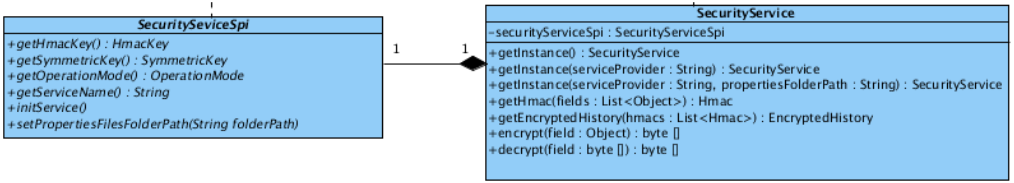
\includegraphics[width=\textwidth]{images/provider.png}
\caption{Representa\c{c}\~{a}o do \textit{provider} da biblioteca} \label{figura:diagramProvider}
\end{center}
\end{figure}

\section{Provider}

\subsection{Remote Callback}

\TODO{uma subseção para isso?}

\section{PKCS\#12 Manager}

\TODO{Ou a seção vai com um nome diferente?}

\section{KeyStore Manager}
%-------------------------------
\chapter{Conclusão}
\label{Conclusão}

TODO

\section{Trabalhos Futuros}

TODO
\bibliographystyle{abnt-alf}
\bibliography{../ref/rfc,../ref/artigo,../ref/references}
%\include{Anexos}
\end{document}

